\documentclass[tikz]{standalone}

\usepackage{tikz}
\usetikzlibrary{trees}
\usetikzlibrary{shapes}
\usetikzlibrary{positioning}
\usetikzlibrary{arrows.meta}

\tikzset{
    mynode/.style = {circle, ultra thick, draw=black, align=center,fill=yellow!30,font=\ttfamily\bfseries\Large,text=black},
    mynoder/.style = {circle, ultra thick, draw=black, align=center,fill=red!30,font=\ttfamily\bfseries\Large,text=black},
    mynodeb/.style = {circle, ultra thick, draw=black, align=center,fill=blue!30,font=\ttfamily\bfseries\Large,text=black},
    mynodeg/.style = {circle, ultra thick, draw=gray, align=center,fill=gray!05,font=\ttfamily\bfseries\Large,text=gray!20},
    mynodegr/.style = {circle, ultra thick, draw=gray, align=center,fill=gray!05,font=\ttfamily\bfseries\Large,text=red},
    edgen/.style = {-,ultra thick,black},
    edger/.style = {-,ultra thick,red},
    edgeb/.style = {-,ultra thick,blue},
    edgeg/.style = {-,ultra thick,gray},
    edgegd/.style = {-,ultra thick,brown,dashed}, % back
    edgevd/.style = {-,ultra thick,violet,dotted}, % forward
    edgexd/.style = {-,ultra thick,blue,densely dotted}, % traversal
    every picture/.style={/utils/exec={\ttfamily\bfseries}},
    every picture/.style={font issue=\ttfamily\bfseries},
    font issue/.style={execute at begin picture={#1\selectfont}}
}

\begin{document}
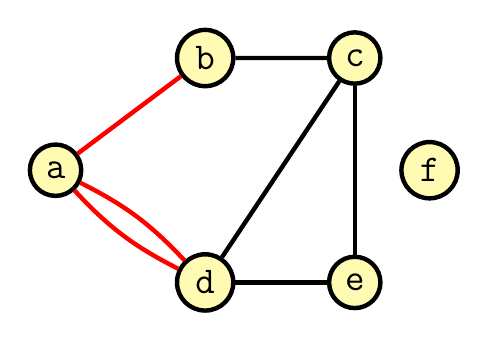
\begin{tikzpicture}[scale=0.95,transform shape]
%
\node[mynode] at (0,0) (a) {a};
\node[mynode] at (2,1.5) (b) {b};
\node[mynode] at (4,1.5) (c) {c};
\node[mynode] at (2,-1.5) (d) {d};
\node[mynode] at (4,-1.5) (e) {e};
\node[mynode] at (5,0) (f) {f};
%
\draw[edger] (a) edge node {} (b);
\draw[edger] (d) edge[bend right=10] node {} (a);
\draw[edger] (a) edge[bend right=10] node {} (d);
\draw[edgen] (b) edge node {} (c);
\draw[edgen] (d) edge node {} (c);
\draw[edgen] (d) edge node {} (e);
\draw[edgen] (e) edge node {} (c);
\end{tikzpicture}
\end{document}